\documentclass[frames]{prosper}
\title{Numerical Solutions of the 2-D Navier-Stokes Equations}
\author{Marvin Washington}
\institution{Jackson State University}
\begin{document}
\maketitle
\begin{slide}{Deformation of the Body}
\begin{figure}
\begin{center}
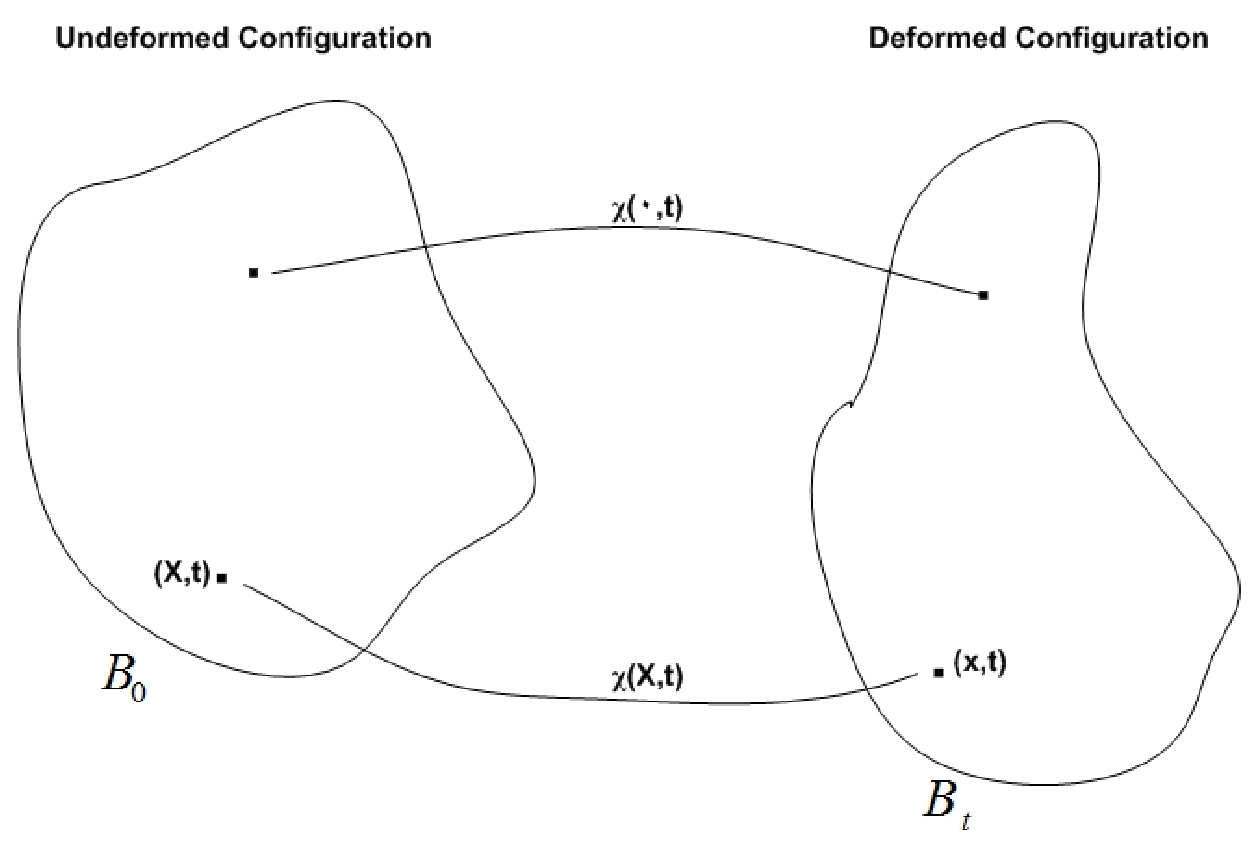
\includegraphics[scale = .3]{config_gragh_marvin.eps}
\end{center}
\end{figure}
\end{slide}

\begin{slide}[Dissolve]{Reynold's Transport Theorem}
$$\frac{D}{Dt} \int_{V} f(\stackrel{\rightarrow}{x},t)dV = \int_{V}\left\{ {\frac{\partial f}{\partial t} + \nabla\cdot(f\stackrel{\rightarrow}{u})}\right\}dV$$
\end{slide}

\begin{slide}[Dissolve]{Conservation of Mass}
The mass of a fluid $(M_{fluid})$ is given by the integral of the fluid density over the fluid domain i.e. \begin{equation} M_{fluid} = \int_{V} \rho(\stackrel{\rightarrow}{x},t)dV \end{equation}
The Conservation of Mass principle states that the derivative of mass w.r.t time must vanish i.e. \begin{equation} \frac{D}{Dt} \int_{V} \rho(\stackrel{\rightarrow}{x},t)dV = 0. \end{equation}
\end{slide}

\begin{slide}[Dissolve]{Conservation of Mass Cont.}
Applying Reynold's Transport Theorem, we have \begin{equation} \frac{D}{Dt} \int_{V} \rho(\stackrel{\rightarrow}{x},t)dV = \int_{V} \left\{\frac{\partial \rho}{\partial t} + \nabla \cdot(\rho \stackrel{\rightarrow}{u})\right\}dV = 0. \end{equation} Since we are working within the confines of the continuum hypothesis and since this equation must hold true for arbitrarily small domains, we can infer that \begin{equation} \frac{\partial \rho}{\partial t} + \nabla \cdot(\rho \stackrel{\rightarrow}{u}) = 0.\end{equation} which is the continuity equation for compressible flows.
\end{slide}

\begin{slide}[Dissolve]{Conservation of Mass Cont.}
$$\frac{D\rho}{Dt} + \rho \nabla \cdot \stackrel{\rightarrow}{u} = 0.$$
which is the continuity equation for compressible flows.\\
in the case where the density remains constant $$\nabla \cdot \stackrel{\rightarrow}{u} = 0$$
is the continuity equation for incompressible flows.
\end{slide}











\begin{slide}[Dissolve]{Conservation of Momentum}
The Conservation of Linear Momentum Principle states that the rate of change of momentum w.r.t time is equal to the sum of the acting forces.
i.e.
$$\int_{V} \rho(\stackrel{\rightarrow}{x},t) \stackrel{\rightarrow}{u}dV = \sum \mbox{acting forces}$$
\end{slide}

\begin{slide}[Dissolve]{Conservation of Momentum Cont.}
Body forces will be expressed as $$ \int_{V} \rho(\stackrel{\rightarrow}{x},t) g(\stackrel{\rightarrow}{x},t)dV $$ and surface forces will be expressed as $$ \int_{\partial V} \sigma(\stackrel{\rightarrow}{x},t)\stackrel{\rightarrow}{n}ds $$
Recasting Newton's $2^{\mbox{nd}}$ law with this in mind yields $$ \frac{D}{Dt} \int_{V} \rho(\stackrel{\rightarrow}{x},t) \stackrel{\rightarrow}{u}dV = \int_{V} \rho(\stackrel{\rightarrow}{x},t) g(\stackrel{\rightarrow}{x},t)dV + \int_{\partial V} \sigma(\stackrel{\rightarrow}{x},t)\stackrel{\rightarrow}{n}ds $$
\end{slide}

\begin{slide}[Dissolve]{Conservation of Momentum Cont.}
Applying Reynold's Transport Theorem to the term on the left yields $$ \int_{V} \left\{\frac{\partial \rho \stackrel{\rightarrow}{u}}{\partial t} + \nabla \cdot \rho \stackrel{\rightarrow}{u}\stackrel{\rightarrow}{u}\right\}dV = \int_{V} \rho(\stackrel{\rightarrow}{x},t) g(\stackrel{\rightarrow}{x},t)dV + \int_{\partial V} \sigma(\stackrel{\rightarrow}{x},t)\stackrel{\rightarrow}{n}ds $$
After applying the Divergence Theorem to the last term and regrouping the equation we arrive at $$ \frac{\partial \rho \stackrel{\rightarrow}{u}}{\partial t} + (\stackrel{\rightarrow}{u} \cdot \nabla)\rho\stackrel{\rightarrow}{u} + \rho\stackrel{\rightarrow}{u}\nabla \cdot \stackrel{\rightarrow}{u} - \rho \stackrel{\rightarrow}{g} - \nabla \cdot \sigma = 0 $$
\end{slide}

\begin{slide}[Dissolve]{Conservation of Momentum Cont.}
The stress tensor $\sigma$ for viscous fluids is defined as $$ \sigma := -pI + \tau := -p + \lambda \mbox{div}(\stackrel{\rightarrow}{u})I + 2\mu\delta. $$ Using this stress tensor, the momentum equation becomes $$ \frac{\partial \rho \stackrel{\rightarrow}{u}}{\partial t} + (\stackrel{\rightarrow}{u} \cdot \nabla)\rho\stackrel{\rightarrow}{u} + \rho\stackrel{\rightarrow}{u}\nabla\cdot \stackrel{\rightarrow}{u} + \mbox{grad}p = (\mu + \lambda)\mbox{grad}(\mbox{div}(\stackrel{\rightarrow}{u})) + \mu\Delta\stackrel{\rightarrow}{u} + \rho\stackrel{\rightarrow}{g} $$

If the fluid being studied is incompressible(i.e $\rho$ = $\rho_{\infty}$ = constant), the momentum equation reduces to $$ \frac{\partial \stackrel{\rightarrow}{u}}{\partial t} + (\stackrel{\rightarrow}{u} \cdot \nabla)\stackrel{\rightarrow}{u} + \frac{1}{\rho_{\infty}}\mbox{grad}p = \frac{\mu}{\rho_{\infty}}\Delta\stackrel{\rightarrow}{u} + \stackrel{\rightarrow}{g} $$
\end{slide}

\begin{slide}[Dissolve]{Conservation of Momentum}
The Conservation of Linear Momentum Principle states that the rate of change of momentum w.r.t time is equal to the sum of the acting forces.
i.e.
$$\int_{V} \rho(\stackrel{\rightarrow}{x},t) \stackrel{\rightarrow}{u}dV = \sum \mbox{acting forces}$$
\end{slide}













\begin{slide}[Dissolve]{Dimensional Analysis}
We obtain a dimensionless quantity by taking the ratio of the dimensional quantity over the reference quantity with the same unit.
Those variable are $\stackrel{\rightarrow}{u}$,$\stackrel{\rightarrow}{x}$,$p$,and $t$ and the associated reference quantities are $V$,$L$,$\rho_{\infty}V^2$, and $\displaystyle{\frac{L}{V}}$.
the dimensionless quantities can be defined as $$\stackrel{\rightarrow}{u}^* := \frac{\stackrel{\rightarrow}{u}}{V}, \stackrel{\rightarrow}{x}^* := \frac{\stackrel{\rightarrow}{x}}{L}, p^* := \frac{p}{\rho_{\infty}V^2}, t^* := \frac{Vt}{L}$$
\end{slide}

\begin{slide}[Dissolve]{Dimensional Analysis Cont.}
Substituting  these new variables into the momentum equation for incompressible flow yields
$$\frac{V^2}{L}\frac{\partial \stackrel{\rightarrow}{u}^*}{\partial t^*} + \frac{V^2}{L}(\stackrel{\rightarrow}{u}^* \cdot \mbox{grad}^*)\stackrel{\rightarrow}{u}^* + \frac{V^2}{L}\mbox{grad}^* p^* = \frac{V\mu}{L{^2}\rho_{\infty}} \Delta^* \stackrel{\rightarrow}{u}^* + \stackrel{\rightarrow}{g}$$
Multiplying through by $\displaystyle{\frac{L}{V^2}}$ yields, $$\frac{\partial \stackrel{\rightarrow}{u}^*}{\partial t^*} + (\stackrel{\rightarrow}{u}^* \cdot \mbox{grad}^*)\stackrel{\rightarrow}{u}^* + \mbox{grad}^* p^* = \frac{\mu}{L\rho_{\infty}V} \Delta^* \stackrel{\rightarrow}{u}^* + \frac{L}{V^2} \stackrel{\rightarrow}{g}$$
\end{slide}

\begin{slide}[Dissolve]{Dimensional Analysis Cont.}
This change of variable introduces two dimensionless quantities which describe properties of the flow
$$Re = \frac{\rho_{\infty}VL}{\mu} \Leftrightarrow \frac{\mbox{inertial forces}}{\mbox{viscous forces}}$$\\
$$Fr = \frac{V}{\sqrt{gL}} \Leftrightarrow \frac{\mbox{inertial forces}}{\mbox{gravitational forces}}$$
\end{slide}

\begin{slide}[Dissolve]{Dimensional Analysis Cont.}
With the introduction of the dimensionless body force $$ \stackrel{\rightarrow}{g^{*}} := \frac{L \stackrel{\rightarrow}{g}}{V^2} = \frac{1}{Fr^2}\frac{\stackrel{\rightarrow}{g}}{\left\|\stackrel{\rightarrow}{g}\right\|} $$ the equation becomes $$ \frac{\partial \stackrel{\rightarrow}{u}^*}{\partial t^*} + (\stackrel{\rightarrow}{u}^* \cdot \mbox{grad}^*)\stackrel{\rightarrow}{u}^* + \mbox{grad}^* p^* = \frac{\mu}{L\rho_{\infty}V} \Delta^* \stackrel{\rightarrow}{u}^* + \stackrel{\rightarrow}{g^{*}} $$
\end{slide}




\begin{slide}[Dissolve]{Finite-Difference Approximations}
$$ (u_{t})_{i}^{j} \approx \frac{u_{i}^{j+1} - u_{i}^{j}}{\delta t} $$ (forward finite difference approximation)
$$ (u_{t})_{i}^{j} \approx \frac{u_{i}^{j} - u_{i}^{j-1}}{\delta t} $$ (backward finite difference approximation)
$$ (u_{t})_{i}^{j} \approx \frac{u_{i}^{j+1} - u_{i}^{j-1}}{2\delta t} $$ (central finite difference approximation)
\end{slide}

\begin{slide}[Dissolve]{Flow in a Lid-Driven Cavity}

\end{slide}

\begin{slide}[Dissolve]{Flow Over a Backward-Facing Step}

\end{slide}

\begin{slide}[Dissolve]{Flow Past an Obstacle}

\end{slide}

\end{document}